\chapter{Terms of Reference}\label{tor}

Terms of reference should be first appendix.
\section{Project Title}\label{tor:title}
A Motion Capture/ Detection Device for Skateboards using an Arduino 101
\section{Project Background}\label{tor:background}
\subsection{Why this project?}\label{tor:whythisproject}
The aim of this project is to create a motion detection device using a microcontroller that can be attached to a skateboard to record when skate tricks are performed. 

The initial motivation of this project was the interest I had in doing and embedded systems project as the general theme for my final year project at university. The topic of embedded systems is something I find particularly interesting. With the amount of smart home technologies cropping up these days (Gartner is predicting a typical family home could contain more than 500 smart devices by 2022, but right now, most consumers see smart home as a nebulous term without a clear value proposition. - Gartner 2015) and the ease in which to get user friendly hardware someone like myself can use, I wanted to create one of my own.  

With this in mind I looked into how I could create something I could use alongside my hobbies. At the time when I was thinking about a ‘Smart’ device I could make I had just started taking up skateboarding. 

From here I wondered if you could use a device to record the distance you have travelled on skateboard, however when it comes to being ‘good’ at skating it is not down to the distance you have travelled but down to tricks you can perform. 

I then started to think about a way of being able to digitally record when a trick has been performed. Which then led me to conclusion that by using a microcontroller as a motion detector you should be able to distinguish each trick due different changes on all 3 axes’ (X, Y and Z).

With the world of Skateboarding not really incorporating technology so far in its lifespan I thought that this would be a good opportunity so see if I could pioneer something myself that would be a use to the community as a whole if they wanted to use it. 

Primarily this project is aimed at developing something for intermediate to advanced skateboarders so that they can record and look at the tricks they have performed over the course of a day skating for example the data could also be used in such a way to record how many tricks a skater has performed over the course of a month or a year. This is something that hasn’t yet been created, I wondered why this hadn’t been tried yet but couldn’t think of a reason why as the logic behind detecting a trick using a motion detector seems sound. 

However, this technology could be useful for Skateboarders regardless of their ability and could actually be of more use to beginners if I developed this project on further to use the data of the motion detector to suggest what the skateboarder needs to do in order to land the trick they are trying to perform.

Following on from this I could expand on the product that completes the initial objectives for this project and use the technology I develop to improve it so that it can use the data to monitor the form of the trick (how well it is executed). This would be something that could be very useful for skateboarding competitions as it will help judges to recognise how well a trick was performed. With skateboarding being accepted into the Olympics as a sport for Tokyo 2020 this kind of technology would be potentially sought after.
\subsection{What issues will I face?}\label{tor:projectissues}
There are several issues that are presented to me be taking on this project. Firstly, I will need to find a place on the skateboard where the microcontroller can go without disrupting the users skating.

The point of doing this project without taking this into consideration would be flawed, having the microcontroller in a bad position could limit skateboarder’s ability to do certain tricks. I couldn’t place the microcontroller on the top of the board as it would make feet positioning difficult which is a major part of performing skateboarding tricks. 

This means that the microcontroller has to go on the bottom of the board, as a result I will have to face the issue of choosing a place on the bottom of the board to put the microcontroller which will firstly protect it from damage on impact of landing tricks but also placed in such a position that all grind tricks can be performed without a problem for the skater.

Another issue as well as a main objective within this project is determining the approach for detecting when tricks are performed. I know that each trick you can perform causes the board to move in a different way and knowing this means in theory it will provide different values when being monitored by a motion detector. 

The problem is that different gradients and different surfaces will cause the motion detector to be at potentially different starting positions each time a trick is performed. I will have to find a way of creating the program in such a way where this does not matter and the trick can be picked up regardless of its starting position. 

The requirements needed of the embedded system that I will create generates issues that I will have to overcome in order to complete this project. A common issue with embedded systems is concurrency. This is something that I will definitely have to look at as I have hardware components on the board running concurrently. 

The microcontroller will have to read the data from the motion detection components as well as maintaining a connection to the mobile device and posting the data to it. This will happen concurrently so I will have to look at solutions to prevent problems such as deadlock and starvation occurring. (Due to the constrains of embedded hardware and use cases of embedded systems, specific concurrency solutions are required.  Schramm and Sabo 2008) This means I will have to evaluate several different approaches specifically to creating concurrent systems and choose which one I will implement based on the specification I set out for the embedded system.

Other common embedded systems I will have to overcome include: making my system reliable, predictable and suited for a real – time environment. These issues will be discussed thoroughly in the Literature review I have to write as part of my project analysis section.
\section{Proposed Work}\label{tor:proposedwork}
\subsection{Sourcing the perfect microcontroller}\label{tor:sourcemicrocontroller}
Before I can begin the development section of this project I need to source an appropriate microcontroller based on two major factors: 
\begin{enumerate}
\item Having all the components I need for the motion detection and communication to a mobile phone. (Accelerometer and/or Gyroscope as well as a Bluetooth Module)
\item Being as small as possible so that it is not taking up too much room on the bottom of the skateboard. 
\end{enumerate}
I will then decide where the microcontroller will be placed on the bottom of the skateboard which subsequently will give me my size specification needed for the microcontroller, leaving me with the task of finding a board of the specified size with all the relevant components I need.

\subsection{Create the Initial Embedded System and Capture Test Data}\label{tor:esandtestdata}
The main challenge of this project is to establish how I will distinguish each skate trick as and when it is performed. This will be done by creating an embedded system to analyse data generated by either an accelerometer, gyroscope or both working together in tandem. I will collect the test data using an open source program called Processing (Processing is a flexible software sketchbook and a language for learning how to code within the context of the visual arts. – Processing Website 2016) This software will draw a graph in real time based on the position of my microcontroller using data produced by the relevant components. 

For this initial test I will be using a serial connection between the PC and microcontroller as this will be the simplest way to get my microcontroller hooked up to the Processing application to start recording data. I will place the microcontroller connected to the PC on a skateboard. Once the device is attached to the skateboard I will replicated the movements of the skateboard performing certain tricks. By doing this I will be able to observe, via the graph drawn by Processing in real time, how the movement caused by each trick affects the data values given by the motion detection components. 

By analysing this data, I will be able to come up with an approach for processing the data when it is posted online so that it can be converted from raw data into a representation of this data in a form of what tricks have been performed and how many times they were performed later on in the project.

By carrying out this section of the project I will be able to evaluate how difficult the project will be too complete.

\subsection{Give the Microcontroller Bluetooth Capability}\label{tor:bluetoothcapability}
Once I am satisfied with the data I have collected, and analysed it enough to come up with a solution to the problem of distinguishing and recording a skate trick, I will take on the task of getting the microcontroller connected to a smartphone device via Bluetooth. This will entail adding to the initial embedded system so that it can use the on-board Bluetooth module to make itself available for connection to a mobile device.

How this will be done will depend on the Microcontroller that I purchase, some microcontrollers already have applications for Android and iOS devices that can be used to control components such as the on-board LED’s. Although I will not be using the LED’s specificity in this project it will give me a good framework for establishing the Bluetooth connection as I can look at the source code for these applications and see how the connection is made.

As a result of this section of work I will have a basis for the mobile application needed for my gateway from the microcontroller to the internet. However, for this section the application will be very basic and its only real function at this point will be to establish a connection from the microcontroller to the mobile device so that I can start working on sending the data from the board back to phone to then be pushed onto the internet.

During this phase of the development I will study the Bluetooth stack protocol so I have a solid understanding of its workings so I can identify any issues that may occur using Bluetooth for the wireless technology involved in this project.

\subsection{Create the Mobile Application Gateway}\label{tor:mobileappgateway}
During this phase of the development I will develop the protocol by which the data will be sent from the microcontroller to the mobile device. Initially I will store the data received by the application into the mobile phones memory so I can view it. From here I will be able to see whether the data is being transmitted to the phone correctly and consistently. It will also show me if there are any differences in the data captured by the board when it is used properly to perform skate tricks rather than just emulating them myself. 

Once I am happy with the way the data is being sent from the board to the phone when properly performing the tricks, I will then create an online database for this data to transferred into. This will require me setting up the database in way dedicated to receiving raw accelerometer or gyroscope readings.

When this database is then set up I will create a method within the mobile application that will post up the data receives from the board up to the internet and store it in the database I create on the web. If an internet connection is not available at the time of data capture, then the data will be saved into the phones memory so that it can then be posted online when a connection becomes available.

\subsection{Presenting the Captured Data}\label{tor:presentingdata}
The final phase of development work to be carried out for this project will be creating a form of web based application that will use the data that is stored in the online database. The web application will be used by the user to view the data that is stored and present in a friendlier way than just raw accelerometer or gyroscope data readings. 

To do this I will use the methods created as a result of the data analysis carried out in the second section to distinguish between each trick and create a method or algorithm to translate the recorded data into presentable values such as “Kick Flip” or “Pop – Shuvit”. To do this I am planning on creating a system in something like PHP or Python, this system will contain a method which will have a way of processing the case of each individual trick for example it could look something like this: 
\begin{figure}
\begin{center}
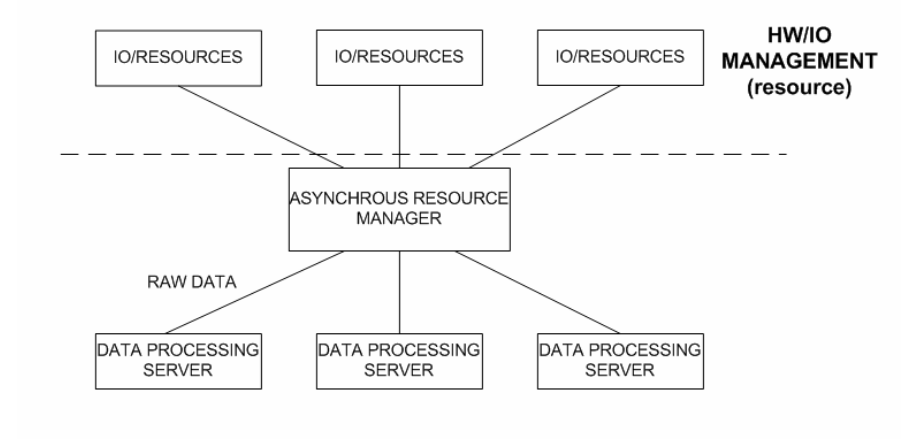
\includegraphics[width=.75\textwidth]{TOR/fig1.png}
\end{center}
\caption{Pseduo Code}
\end{figure}
I will use this sort of method so the application will be able to handle different tricks performed on the skateboard. Once I am satisfied that the method can interpret the data properly it is time to design the user interface, this will require me to brush up on some basic UI and UX skills learnt in my previous 2 years of university. I would like the development of this project to be of use to other people as well so making this web based application well designed is important.

\section{Project Aims}\label{tor:projectaims}
\begin{enumerate}
\item To investigate whether a motion detector can be used to record and define Skateboarding tricks as and when they are performed.
\item To create a mobile phone application which can receive data from a paired microcomputer that is attached to a Skateboard via Bluetooth. This application will display the data it receives in a user friendly manner.
\end{enumerate}

\section{Project Objectives}\label{tor:projectobjectives}
\begin{enumerate}
\item To write a literature review on the issues presented to me by creating an embedded system and what solutions I can use to overcome these problems. 
\item To establish a method for how I can distinguish between different skateboarding tricks using the accelerometer and gyroscope.
\item Gather a thorough set of requirements to specify what the application and microcontroller are able to do when working in tandem. 
\item To create an embedded system which can use a microcontroller to produce readings of raw data. 
\item To establish a wireless protocol by which I can communicate this raw data produced by the microcontroller to a mobile phone. 
\item Design user interfaces for all of the mobile application’s use case scenarios based on the requirements I capture.
\item To create an application for mobile phone’s which uses the data received wirelessly from the microcontroller and presents this to users in an interactive way based on the requirements I capture. 
\item Evaluate the microcontroller’s ability to be used as a device to detect when skateboarding tricks have been performed. 
\item Evaluate the performance of the application created to pair with the microcontroller and use the data it receives from it to present it user interactively. 
\item Evaluate my performance during the course of developing this product and project as a whole including coding, time management skills and ability to work according to a schedule.
\end{enumerate}

\subsection{Learning Objectives}\label{tor:learningobjectives}
\begin{enumerate}
\item Investigate and understand what makes for good UI and UX then apply this to my mobile application development process. 
\item To learn and understand how to transmit information wirelessly via Bluetooth and how to establish secure and reliable protocols for doing this.
\end{enumerate}

\section{Skills Required}\label{tor:skillsrequired}
\begin{longtable}{| p{.2\textwidth}|p{.3\textwidth}| p{.3\textwidth} | p{.3\textwidth}|}[h]
%\begin{tabular}
\hline
\textbf{Skill} & \textbf{Level of experience with this skill} & \textbf{Do I need to Improve this skill} & \textbf{How will I improve this skill} \\
\hline \hline
Researching for relevant literature &
Moderate &
Yes & Read up on research methods as well as working on the search criteria that I use to find references.\\
\hline
Requirements Gathering &
High &
No & Not applicable. \\
\hline
Data Analysis &
Moderate &
Yes & I have to look at trends previously when studying subjects such as statistics. I will improve this technique solely by gathering data for my project and looking at it and trying to determine what is means. \\
\hline
Creation of embedded systems &
High &
Yes & I am comfortable with the workings of embedded systems although I do believe I need to improve on this further for this project. \\
\hline
Mobile Application Development &
Moderate &
Yes & I will improve this skill through dedicating time to studying the development of mobile applications and apply this to my project. \\
\hline
Project and Time Management &
High &
Yes & Even though I am already competent in this skill, I believe I willimprove even further as I have never had to manage a project of this scale.\\
\hline
Working with wireless communication &
Low &
Yes & I have never worked with wireless communication before in any sense so this will be a whole new experience for me. I will learn this through studying methods of transferring data online and reading literature. I will also be able to reference the microcontrollers function library’s for wireless components.\\
\hline
Evaluation &
High &
No & Not applicable
%\end{tabular}
\caption{Using the \texttt{tabular} environment\label{device:table}}
\end{longtable}

\section{Bibliography}\label{tor:bibliography}
Add References here

\section{Resources}\label{tor:resources}
\subsection{Hardware}\label{tor:hardware}
\begin{itemize}
\item A Microcontroller to be used as a motion detector
\item A laptop to install IDE on for programming the application and embedded system
\item Smartphone to install and test the application on
\item A skateboard to attach the microcontroller to
\end{itemize}
\subsection{Software}\label{tor:software}
\begin{itemize}
\item IDE for mobile application development
\item A software called Processing which will present accelerometer readings from the microcontoller for me
\item The Arduino development environment for writing the embedded system
\item LaTeX for producing all documents
\item MS Project for creating my project plan
\item Adobe Illustrator for designing the application screens
\end{itemize}

\section{Report Structure and Contents}\label{tor:reportstruct}
\subsection{Title Page}\label{tor:rpttitlepage}
\subsection{Contents Page}\label{tor:rptcontentspage}
\subsection{Abstract}\label{tor:rptabstract}
The abstract will outline the project as whole. It will briefly mention the aims of this project and what work I have carried out in order to meet these aims. I will mention the methodology approach to the project and briefly mention the end result of the project.
\subsection{Introduction}\label{tor:rptintro}
This section will discuss the reasoning for carrying out the project and outline the approach I will take for the development and what deliverables I will satisfy. The introduction will also outline what the other sections of the report will include.
\subsection{Analysis}\label{tor:rptanalysis}
This section will be made up of 2 chapters. The first will be a literature review which will discuss the key issues I will face during the development of this project and evaluate the solutions to these problems in a critical way.
\subsubsection{Literature Review}\label{tor:rptlitreview}
Within my literature review I will discuss 2 topics relevant to the work I am carrying out for this project. (Covers Objective 1).
\subsubsection{Embedded System Design Challenge}\label{tor:rptesdesign}
In this section of the literature review I will discuss the main challenges and choices that need to be made when creating embedded systems. I will evaluate the different approaches for concurrency, scheduling etc. and explain the choices of methods I am going to use.
\subsubsection{The Hardware}\label{tor:rpthardware}
This section will justify my hardware decisions.
\subsubsection{Machine Learning Techniques}\label{tor:rptmachinelearning}
I also discuss pattern recognition with digital signal processing evaluating the techniques I have available to me and which one will be best suited to the work needed for my project. (Detecting the skateboard tricks).
\subsubsection{Requirements Commentary}\label{tor:rptrequirments}
The second chapter of this section will be discussion of the project requirements justifying where necessary and explaining how I captured the requirements. (Covers Objective 3).
\subsubsection{Methodology Approach}\label{for:rptmethodologyapproach}
I will discuss my methodology approach for this project comparing different approaches you can take and explaining why the approach I decided to take was the correct one for the development of this project.
\subsection{Synthesis}\label{tor:rptsynthesis}
\subsubsection{Deliverables Commentary}\label{tor:rptdeliverables}
In this section I will be discussing why the deliverables of the project are required for its completion.
\subsubsection{Skate Trick Detection Analysis}\label{tor:rptskateanalysis}
An explanation of the process I went through to coin a method to detect when and which skateboardin trick have been performed. (Covers objectives 2).



